
\section{Analyse de VFC}
\subsection{Analyse des fonctions de magnitudes}
Les paramètres des fonctions de magnitude $m_1(x,y)$ et $m_2(x,y)$ du noyau de convolution $\mathbf{k}$ ont une influence importante sur la convergence du contour actif vers les contours d'intérêt.

\paragraph*{Paramètre $\gamma$ de $m_1(x,y)$}
L'évolution du profil de la fonction $m_1(x,y)$ en fonction de $\gamma$ (\ref{gamma}) permet de voir le poids important appliqué aux bords du noyau de convolution lorsque $\gamma$ diminue. Cela à pour conséquence d'accroitre la portée de convergence des contours d'intérêts comme le montre la figure \ref{fig:gamma} en annexe pour des valeurs faibles de $\gamma$. Au contraire, une valeur trop élevée diminue fortement la portée de convergence du contour d'intérêt. 

\paragraph*{Paramètre $\sigma$ de $m_2(x,y)$}
On peut voir la fonction $m_2(x,y)$ comme une gaussienne d'écart type $\sigma$. Ainsi, plus $\sigma$ augmente, plus les poids appliqués au noyau de convolution sont importants comme le montre le profil de $m_2(x,y)$ en fonction de $\sigma$ (\ref{sigma}). Cependant, on peut voir que le choix de sigma est lié à la taille du noyau de convolution $R$. En effet, si $\sigma$ est trop important, un point quasi-uniforme sera appliqué sur tout le noyau de convolution. 

\begin{figure}[!h]
   
   \begin{subfigure}[c]{.5\linewidth}
     \centering
     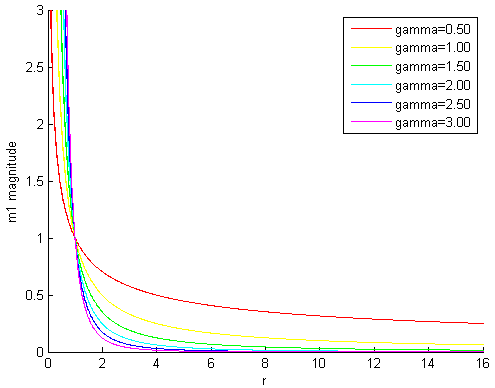
\includegraphics[scale=0.5]{Chapters/Images/graph_m1.png}
     \caption{}
     \label{gamma}
   \end{subfigure}
   \begin{subfigure}[c]{.5\linewidth}
     \centering
     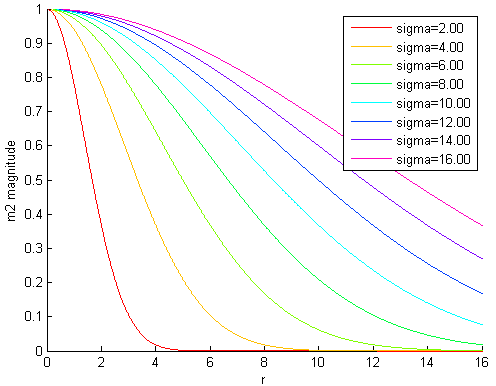
\includegraphics[scale=0.5]{Chapters/Images/graph_m2.png}
     \caption{}
     \label{sigma}
   \end{subfigure}\\
   
   \caption{Profil des fonctions de magnitude  $m_1(x,y)$ (a) et $m_2(x,y)$ (b) en fonction de $\gamma$ et $\sigma$ .}
   \label{fig:profil}
\end{figure}

\subsection{Taille du noyau de convolution}



\subsection{Convergence sur des contours concaves}
Une des principales améliorations introduites par GVF est la convergence des contours actifs dans les concavités de l'objet d'intérêt. La nouvelle force externe introduite par Bing Li et al. (\cite{vfc}) est censée conserver ces propriétés de convergences. Nous avons donc décidé de tester la bonne convergence d'un contour actif et de comparer les résultats obtenus en utilisant GVF et VFC.

Pour réaliser ces tests, nous avons donc choisi deux images de test synthétiques. La première est une étoile, la seconde est représentée par un carré dont un bord a été retiré (voir annexe \ref{ann_synthetic_star_square}). L'initialisation des contours actif est la même pour les deux forces externes, et les paramètres choisis ont été les suivants :\\

VFC : $R = 128$, force $m_{1}$ avec $\gamma = 1.7$\\
GVF : $\mu = 0.2$, $nb_{iter} = 10000$\\

Les images sont présentés en annexe (annexe  \ref{ann_concavities_results}). On peut remarquer que dans le cas des deux forces externes, les contours actifs ont bien convergé dans les différentes concavités des objets d'intérêt. D'autre part, le nombre d'itération nécessaire pour converger est à peu près le même dans les deux cas. Cependant, il est important de noter que le temps de calcul des deux forces externes est très différent. En effet, pour que la force externe GVF soit capable de converger, il a fallu prendre un nombre d'itération de 10000. En pratique, le calcul de la force externe VFC a été 160 fois plus rapide que celui de GVF. Cette spécificité est d'ailleurs mise en valeur dans \cite{vfc}. 

\subsection{Robustesse à l'initialisation du contour}
D'après \cite{vfc}, VFC se comporte très bien en ce qui concerne l'initialisation du contour actif. Nous avons voulu tester cette déclaration. Nous avons donc lancé l'algorithme avec différentes initialisations. Les résultats sont présentés dans l'annexe \ref{ann_init_results}.\\ 

Les résultats montrent que malgré une bonne convergence pour des initialisations centrées approximativement au milieu de l'étoile, la convergence ne se fait pas dans le cas ou le contour actif est placé préférentiellement sur un des bord des lignes de courant. Cela met en valeur l'intérêt d'ajouter une énergie de contrainte $E_{contraintes}$ comme défini dans \cite{kaas}. 


\subsection{Robustesse à différents type de bruit}
La force externe VFC a été introduite afin de réduire la sensibilité des contours actifs au bruit. Nous avons donc décidé de comparer les résultats obtenus en utilisant GVF et VFC en présence de différents types de bruit. \cite{vfc} précise que GVF est spécialement sensible à un bruit impulsionnel. Nous avons donc choisi de tester l'influence de ce bruit. Nous avons aussi testé l'évolution des deux forces en présence d'un bruit additif gaussien. 

Les images sont présentées en annexes (\ref{ann_noise_results}). On peut remarquer qu'effectivement, la force externe GVF se comporte très mal en présence d'un bruit impulsionnel. Avec uniquement 5\% des pixels touchés, les contours ne convergent pas vers l'étoile. Avec 10\% le contour initial n'est presque pas déformé. A l'inverse, VFC converge très rapidement. Même avec 15\% de pixels touchés, on obtient des résultats convaincants. Les bout des étoiles sont cependant moins bien définis par le contour actif.\\

Dans le cas d'un bruit additif gaussien, GVF ne se comporte pas très bien non plus. En revanche, on remarque que VFC ne fait pas beaucoup mieux. Les contours actifs sont bien attirés vers les bords de l'étoile dans un premier temps. Cependant, le bruit présent à l'intérieur de l'étoile cumulé avec la force interne des contours entraîne une contraction du contour actif.\\

On peut remarquer qu'avec une taille de noyau plus petit ($R = 64$), le contour actif converge mieux vers les contours. On peut donc se demander si la portée de convergence doit être la même pour tout les points de l'image. Cette question sera abordée dans le dernier chapitre.
